% Gemini theme
% https://github.com/anishathalye/gemini
%
% We try to keep this Overleaf template in sync with the canonical source on
% GitHub, but it's recommended that you obtain the template directly from
% GitHub to ensure that you are using the latest version.

\documentclass[final]{beamer}

% ====================
% Packages
% ====================

\usepackage[T1]{fontenc}
% \usepackage[utf8]{inputenc}
\usepackage{lmodern}
\usepackage[size=custom,width=150,height=90,scale=1.0]{beamerposter}
\usetheme{gemini}
\usecolortheme{gemini}
\usepackage{graphicx}
\usepackage{subfig}
\usepackage{booktabs}
\usepackage{tikz}
\usepackage{pgfplots}

\usepackage{lipsum}
\setbeamertemplate{caption}[numbered]

% ====================
% Lengths
% ====================

% If you have N columns, choose \sepwidth and \colwidth such that
% (N+1)*\sepwidth + N*\colwidth = \paperwidth
\newlength{\sepwidth}
\newlength{\colwidth}
\setlength{\sepwidth}{0.024\paperwidth}
\setlength{\colwidth}{0.22\paperwidth}

\newcommand{\separatorcolumn}{\begin{column}{\sepwidth}\end{column}}

% ====================
% Title
% ====================

\title{Mantle convection under the South American plate \\and possible implications on the evolution of the Pantanal Basin}

\author{Jamison Assunção \and Victor Sacek}

\institute[shortinst]{Department of Geophysics, Universidade de São Paulo\\ Instituto de Astronomia, Geofísica e Ciências Atmosféricas}

% ====================
% Body
% ====================

\begin{document}

% ====================
% Logos
% ====================

\addtobeamertemplate{headline}{} 
{\begin{tikzpicture}[remember picture,overlay] 
\node [shift={(-28cm,-7cm)}] at (current page.north east) {\includegraphics[height=9cm]{figures/usp-logo-png.png}}; 
\end{tikzpicture}
\begin{tikzpicture}[remember picture,overlay] 
\node [shift={(-13cm,-7cm)}] at (current page.north east) {\includegraphics[height=7cm]{figures/iagcompasso_V.png}}; 
\end{tikzpicture}
\begin{tikzpicture}[remember picture,overlay] 
\node [shift={(17cm,-7cm)}] at (current page.north west) {\includegraphics[height=7cm]{figures/logo-isag.png}}; 
\end{tikzpicture}}
% \begin{tikzpicture}[remember picture,overlay] 
% \node [shift={(35.5cm,-7cm)}] at (current page.north west) {\includegraphics[height=7cm]{figures/graphic_egu_photo_yes.png}}; 
% \end{tikzpicture}}

% ====================
% Poster
% ====================

\begin{frame}[t]

\begin{columns}[t]
\separatorcolumn

\begin{column}{\colwidth}
  \begin{block}{Introduction}

    The Pantanal wetland (Figure \ref{fig:pantanal-basin}) is a Quaternary basin in Southwestern Brazil, reaching up to $\sim500$ m of sedimentary package. Although the relatively recent formation of the basin, the mechanisms involved in the origin of the regional subsidence are not fully understood. Previous works proposed a flexural origin for the basin, invoking the last pulse of Andean tectonism and consequent topographic load as the source for the creation of the Pantanal Basin. However, taking into account the flexural rigidity of the South American lithosphere and the Andean geometry, it is difficult to explain the subsidence amplitude as well as the position of the basin due to flexural effects. Therefore, probably another mechanism must be involved in the formation and evolution of this active sedimentary basin. 

    \begin{figure}
        \centering
        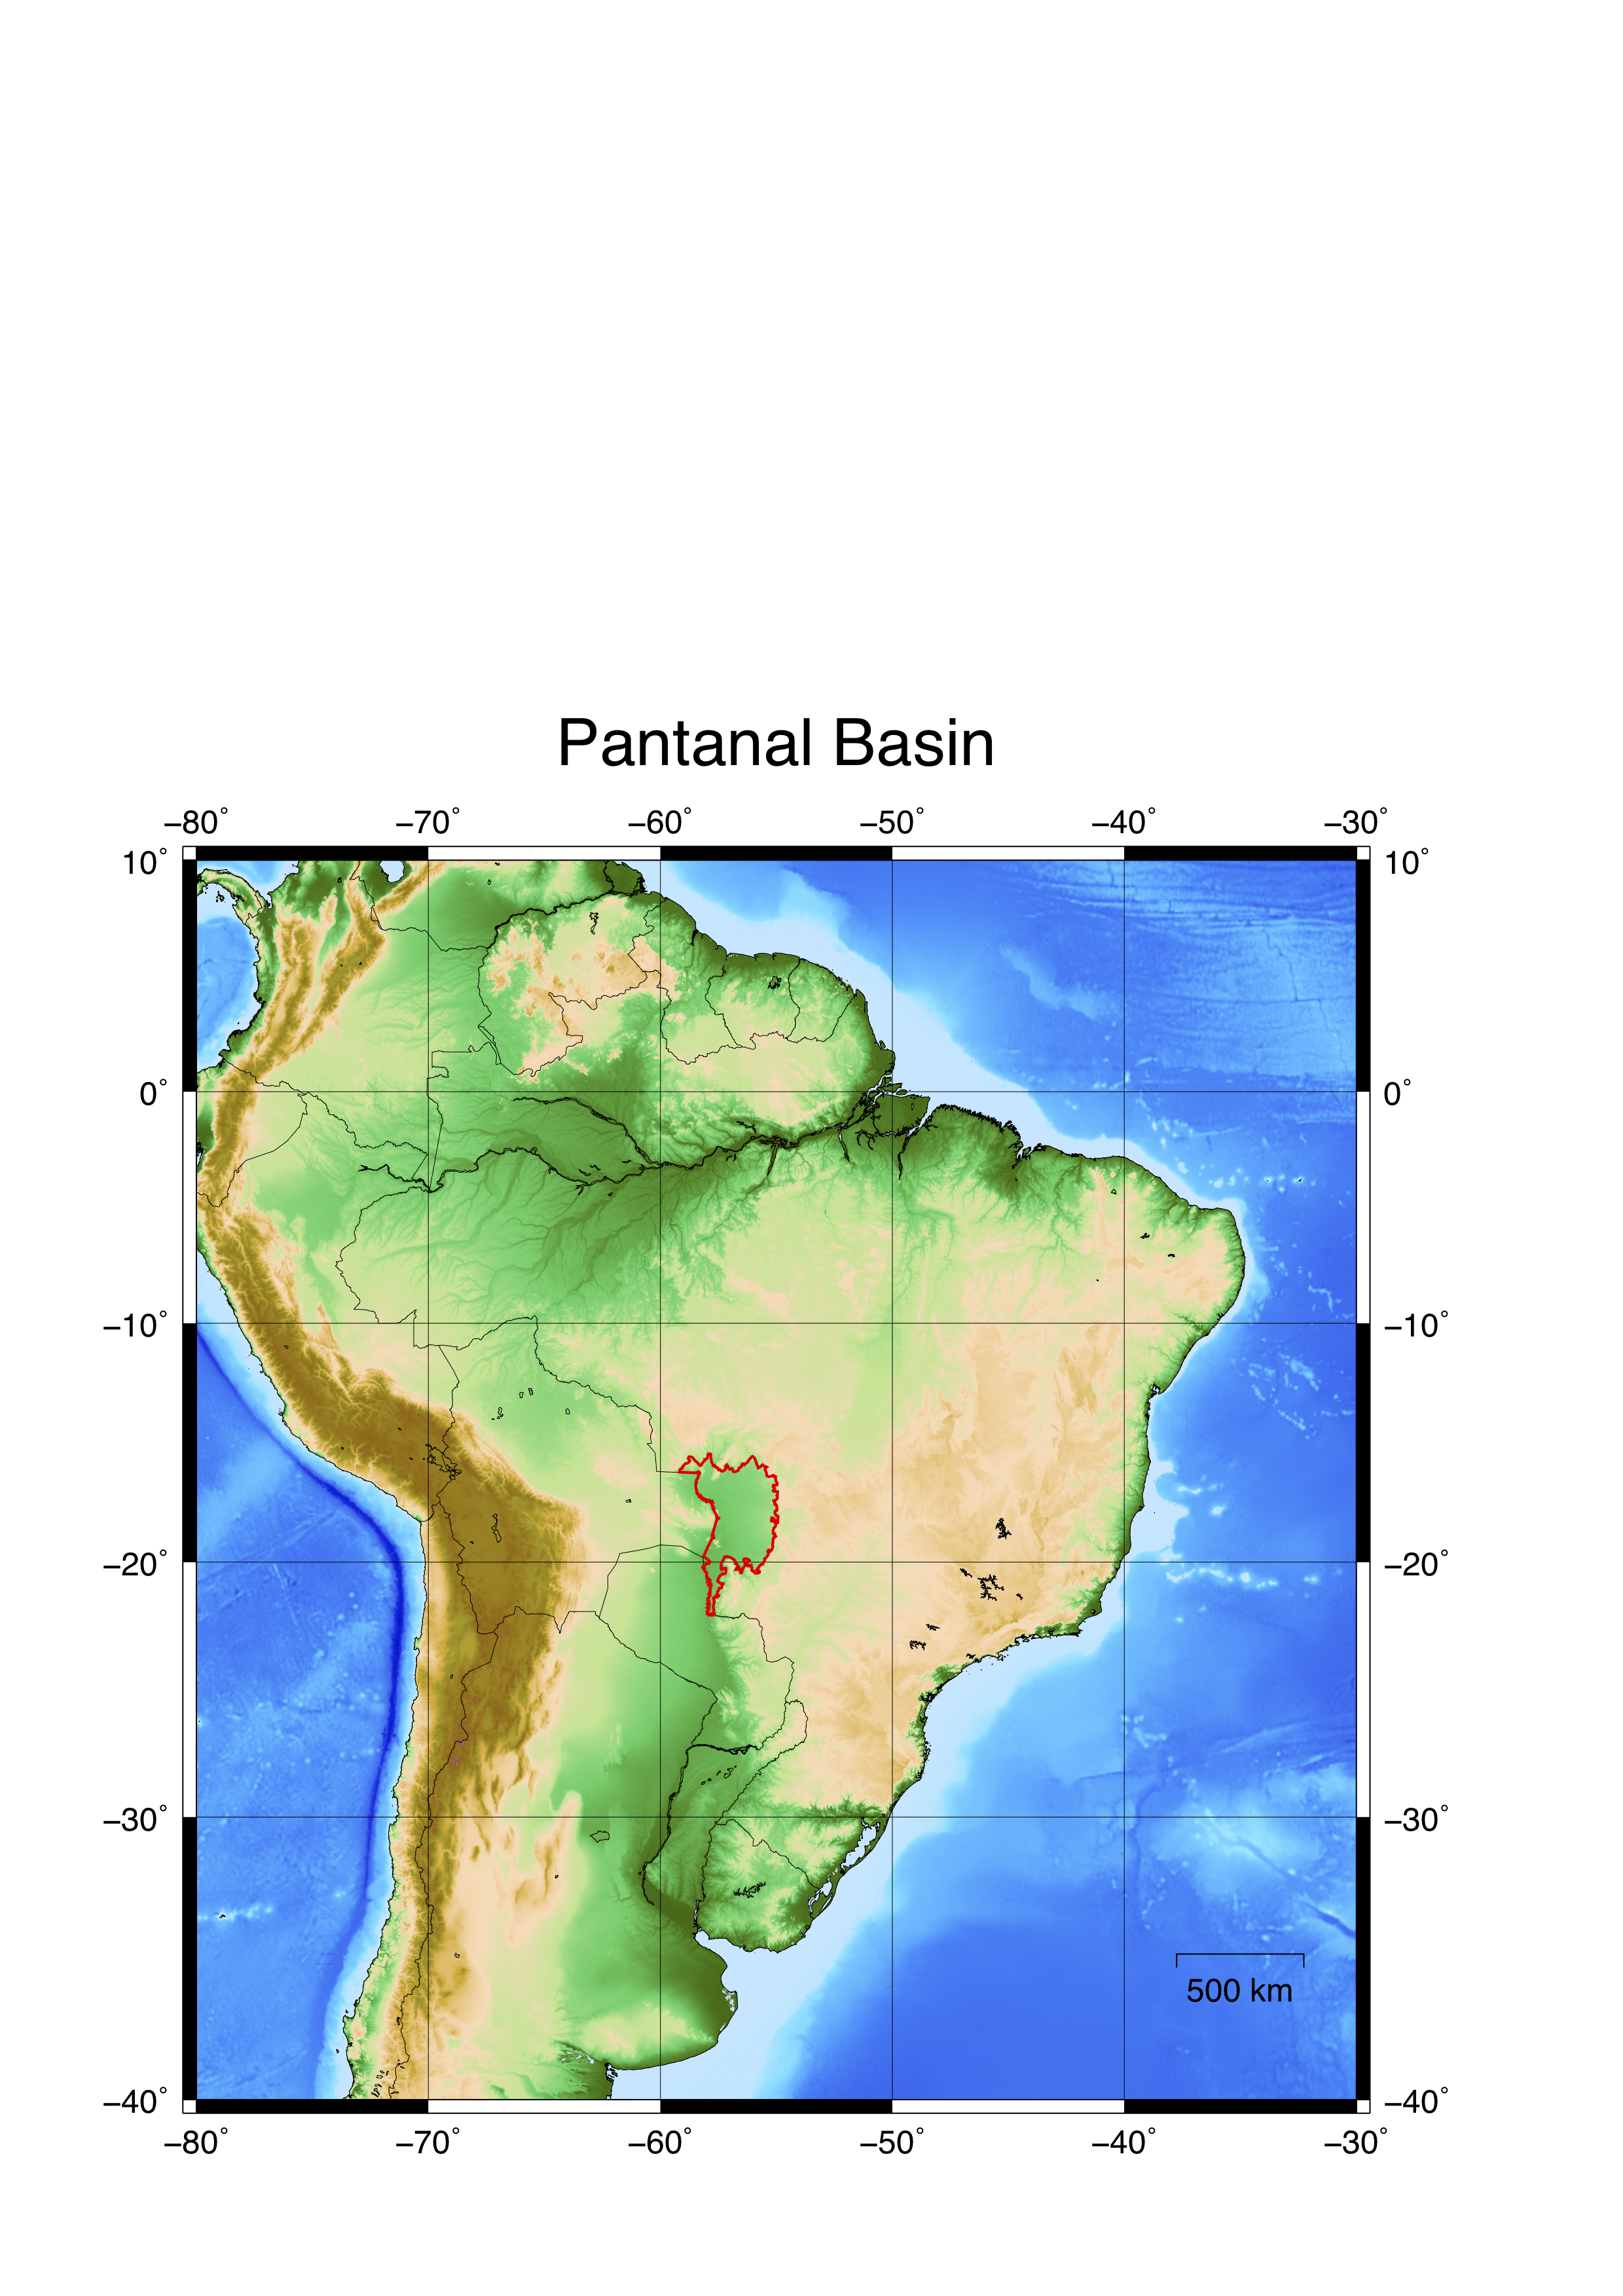
\includegraphics[trim={1.5cm 1.5cm 2cm 10cm},clip,scale=1]{figures/south-america+pantanal.png}
        \caption{ Map of South America showing the Pantanal Basin perimeter.}
        \label{fig:pantanal-basin}
    \end{figure}

    In the present work we will perform several 2D numerical simulations to evaluate how initial conditions can contribute to the buoyancy of the subducting Nazca plate. The results will be used in an upcoming study to calculate the influence of mantle convection generated by the subducting slab geometry and assess if it can induce dynamic topography and contribute to create the depression associated with the Pantanal Basin. 

    We used a finite element code to simulate the thermochemical convection in the mantle, calculating the associated dip angle of subduction along a profile from 80.0ºW to 48.5ºW, crossing the Pantanal wetland at a latitude of 18ºS. To simulate the mantle flow, the thickness of both lithosphere and crust were resampled from the global LITHO1.0 model and the initial thermal structure for subducting slab was constructed based on a simplified thermokinematic model. The subducting slab geometry adopted was derived from the Slab2 model. The results will be considered to three dimensional models in the future to better represent latitudinal variations of the subducting slab and consequently improve the representation of the dynamic topography in the interior of the South American Plate. 
    
    % We propose that, although the wavelength of the negative dynamic topography produced in the interior of the continent is larger than the width of the Pantanal basin, the amplitude of the subsidence and the geographic position of the depression are compatible to the observed values. 
    
    % Additional three dimensional models will be considered in the future to better represent latitudinal variations of the subducting slab and consequently improving the representation of the dynamic topography in the interior of the South American Plate. 

  % \end{block}
  
  
  
    % The origin of the foreland Pantanal basin in Southwestern Brazil is not fully understood, but recent studies suggest it developed as a result of the flexural extension of the upper crust due the last pulse of the Andean tectonism \cite{ussami1999basement}. However, observed shallow and reverse faulting events are incompatible with such an extensional mechanism \cite{assumpccao1988source}. It is also a discussion topic if the basin is currently situated on the fore-bulge, as flexural models suggest \cite{ussami1999basement}, or if it rests on the back-bulge, from where its sediment content is typical \cite{horton1997modern}.
    
    
    
    % Taking into account the flexural rigidity of the South American lithosphere and the Andean geometry, we are prone to believe there is another mechanism involved in the subsidence of the Pantanal basin besides the flexural. Therefore, a numerical simulation is needed to study the convecting-mantle influence on the evolution of the basin. 

    %For the model problem, it is necessary to resort to reasonable initial conditions and boundary conditions. Said that, it is extremely important to study the limitations posed when choosing a layer model, build a velocity field, establish an initial temperature structure, and choose a rheological model to represent the intrinsic parameters of the material.
    
    % This work will test several initial conditions when simulating thermochemical convection of the mantle. The results will be discussed focusing on how these initial conditions affect the buoyancy of the subducting Nazca plate under the South America plate. This study will be a reference for an ongoing numerical study of the area, which in turn will calculate the contribution of the dynamic topography and evaluate the mantle influence on the current observed subsidence of the basin, as well as compare it against residual topography maps.
    
  \end{block}

  \begin{block}{Numerical Methods}

    We used the 3D finite element numerical code MD3D \cite{sacek2017post} to solve the Stokes flow for a fluid using the Boussinesq approximation in a Cartesian coordinate system. This resulted in the equations for conservation of mass (Equation \ref{mass-conservation}), momentum (Equation \ref{momentum-conservation}) and energy (Equation \ref{energy-conservation}) \cite{treatise7.05}.
    \begin{equation}{\label{mass-conservation}}
        u_{i,i}=0
    \end{equation}
    \begin{equation}{\label{momentum-conservation}}
        \sigma_{ij,j}+g\alpha \rho_0 T \delta_{i3} = 0
    \end{equation}
    \begin{equation}{\label{energy-conservation}}
       \frac{\partial T}{\partial t}+u_{i}T_{,i}=\kappa T_{,ii}
    \end{equation}
    where $u_i$ is the velocity in the $i$ direction, $\sigma_{i,j}$ is the stress tensor (Equation \autoref{stress-tensor}), $g$ is the acceleration of gravity, $\rho_{0}$ is the mantle reference viscosity, $\alpha$ is the coefficient of thermal expansivity, $T$ is temperature, $\delta_{ij}$ is the Kroenecker delta function, $t$ is time, and $\kappa$ is the thermal diffusivity. %Where $u_{i}$ represent $\sum_{i}u_{i}$, $u_{,i}$ represents the partial derivative $\partial u/\partial x_{i}$, and ${T_{,ii}}$ represents $\partial^2T/\partial x_{i}^{2}$.
    \begin{equation}{\label{stress-tensor}}
        \sigma_{ij,j}=-P\delta_{ij}+\eta(u_{i,j}+u_{j,i})
    \end{equation}
    where $P$ is the dynamic pressure, and $\eta$ is the viscosity.
    
  \end{block}
  
\end{column}

\separatorcolumn

\begin{column}{\colwidth}
  
  \begin{block}{Initial conditions}
  
  To study how the buoyancy changes as a function of the initial parameters, the length of the subducting oceanic lithosphere will be reduced to match the depth of $450$ km and we will simulate for $5$ Myr until it "recovers its original length. This will serve as well to allow flow beneath the subducting plate, restricted to the longitudinal direction.
  
  \heading{\textcolor{darkblue}{Layer model}}
    The chosen layer model for the simulations is a combination of the Slab2 model \cite{hayes2018slab2} and the LITHO1.0 model \cite{pasyanos2014litho1} (Figure \ref{fig:interfaces}). While the Slab2 provides data for the geometry of the subducting slab, the LITHO1.0 provides information about the thickness of the crust and the depth of the lithosphere-asthenosphere boundary (LAB). 
    \begin{figure}
      \centering
      \includegraphics[width=0.22\paperwidth]{figures/interfaces.png}
      \caption{Example of an initial layer model with minimum LAB depth of $100$ km in the continental regions and maximum oceanic crust depth of $7$ km.}
      \label{fig:interfaces}
    \end{figure}
  \heading{\textcolor{darkblue}{Thermal structure}}
    The lithosphere temperature is assumed to increase with depth for both continental and oceanic regions. It starts at $0$ºC at the surface and increases linearly until $1300$ºC at the bottom of the lithosphere. For the asthenosphere, the geothermal gradient respects the adiabatic relation shown in Equation \ref{adiabtic_curve}.
    \begin{equation}{\label{adiabtic_curve}}
      T(z)=(T_0-273.15)\exp{\frac{\alpha g z}{C_p}}
    \end{equation}
   \noindent where $T_0$ is the potential temperature of the mantle on the surface, $\alpha=3.28\cdot 10^{-5}$ K$^{-1}$ is the thermal expansion coefficient, $g=9.8$ m/s$^2$ is the gravity acceleration, and $C_p=1250$ m$^2$/K s$^2$ is the heat capacity. $T_0$ is defined such that the temperature on the bottom of the model is $1518.68$ºC. This value is chosen to make the viscosity at that depth equals to $10^{19}$ Pa s.
    
   For the subducting oceanic slab, we consider a semi-infinite slab of velocity $v$ descending into an isothermal mantle and solved Equation \ref{energy-conservation} for $\partial T/\partial t=0$. Furthermore, we added a contribution $\delta T = T(z)-T_0$, which is the difference between the potential temperature of the mantle on the surface and the temperature $T(z)$ at a certain depth $z$.
   
   To simulate the heat conduction during before the simulation, we diffused the thermal structure for $20$ Myr using the boundary condition of $\partial T/\partial x=0$ on the sides of the model.
    % Use the command \newline at the end of a line to force justification (and stretch) of that line

\heading{\textcolor{darkblue}{Velocity field}}
        
  The imposed velocity field does not allow normal velocities on the bottom and on the surface of the model. On the sides, the velocity is chosen to cause the oceanic lithosphere to move with velocity $v$ towards the continent. In the asthenosphere, this velocity decreases to zero with the error function. Because of Equation \ref{mass-conservation}, a velocity field is defined to the other side of the model, but with maximum velocity at the bottom, decreasing to zero with the error function and being null for the continental lithosphere.

  A velocity field was also defined for the surface of the model, where the velocity of the oceanic lithosphere was set to be constant and equal to the normal velocity $v$. For the continental lithosphere, we set the velocity to be zero, as the subducting slab should move relative to it. Because the slab would anchor in the continental lithosphere during the subduction, we also set a constant velocity $v$ for the first $200$ km of the continental lithosphere. Although this distance seems big, the dip angle of the subducting slab is small.
        
  \end{block}

\end{column}

\separatorcolumn

\begin{column}{\colwidth}
    \begin{block}{Initial conditions - continuation}

    \heading{\textcolor{darkblue}{Rheology model}}
    
      The viscosity will be considered to vary exponentially as a function of the temperature $T$ and a compositional factor $C$ as in the Frank-Kamenetskii approximation (Equation \ref{rheology-expression}). We consider the mantle to be a fluid of variable viscosity for a steady state ductile creep, as it is usually considered for thermochemical convection \cite{solomatov2000scaling}.
      \begin{equation}{\label{rheology-expression}}
          \eta(T,C) = C\eta_r b^* \exp{(-\gamma T)}
      \end{equation}
      \noindent where $\eta_r$ is the reference viscosity, $b^*$ and $\gamma=E_{a}/RT_{b}^{2}$ are constants and where $E_a$ is the activation energy, $R$ is the gas constant, and $T_b$ is the basal temperature.
    \end{block}

  \begin{block}{Results}

  % The results shown below are those considered to be the most interesting for the series of simulations. 

  % For all the simulations, the movement was predominantly happening in the subducting slab.

  % The three figures below show the subducting slab and the evolution of the curvature of the slab until $5$ Myr. Temperature and velocity profiles were simulated with thicknesses of $80$ km for the subducting slab, and $7$ km for the oceanic crust. The compositional factors are $C = 1000$ for the lithosphere, $C=1$ for the mantle, and $C=0.01$ for the lubricant layer. Densities are $\rho_m=3300$ kg/m$^3$ for the mantle, $\rho_{cc}=2750$ kg/m$^3$ for the continental crust, and $\rho_{oc}=2800$ kg/m$^3$ for the oceanic crust.

  \begin{figure}
		\centering
  		\subfloat[Thermal structure and velocity field at $0.00$ Myr.\label{fig:a}]{\includegraphics[width=0.22\paperwidth]{figures/angle-step_0.png}}\\
  		\subfloat[Thermal structure and velocity field at $2.50$ Myr.\label{fig:b}]{\includegraphics[width=0.22\paperwidth]{figures/angle-step_199.png}}\\
  		\subfloat[Thermal structure and velocity field at $4.99$ Myr.\label{fig:c}]{\includegraphics[width=0.22\paperwidth]{figures/angle-step_363.png}}
  \caption{Temperature and velocity profiles showing the evolution of the dip angle of the subducting slab until $4.99$ Myr. The simulation was made using a thicknesses of $85$ km for the subducting slab, and $6$ km for the oceanic crust. The compositional factors are $C = 1000$ for the lithosphere, $C=1$ for the mantle, and $C=0.01$ for the lubricant layer. Densities are $\rho_m=3300$ kg/m$^3$ for the mantle, $\rho_{cc}=2750$ kg/m$^3$ for the continental crust, and $\rho_{oc}=2800$ kg/m$^3$ for the oceanic crust.}
  \label{fig:result1}
  \end{figure}
  
  \begin{figure}
    \centering
    \includegraphics[width=0.22\paperwidth]{figures/angle-step_204.png}
    \caption{Simulation with the smallest dip angle difference between the Slab2 and the simulation at $4.98$ Myr. The thicknesses of the subducting slab and the oceanic crust are $80$ and $7$ km, respectively. The compositional factors are $C = 1000$ for the lithosphere, $C=1$ for the mantle, and $C=0.01$ for the lubricant layer. Densities are $\rho_m=3300$ kg/m$^3$ for the mantle, $\rho_{cc}=2750$ kg/m$^3$ for the continental crust, and $\rho_{oc}=2800$ kg/m$^3$ for the oceanic crust.}
    \label{fig:result4}
  \end{figure}

  \end{block}

 \end{column}

\separatorcolumn

\begin{column}{\colwidth}

  \begin{block}{Conclusions}

    \begin{figure}
		\centering
  		\subfloat[$\sim2.5$ Myr.\label{fig:conclusion1}]{\includegraphics[width=0.10\paperwidth]{figures/corr_25.png}}\qquad
  		\subfloat[$\sim 5.0$ Myr.\label{fig:conclusion2}]{\includegraphics[width=0.10\paperwidth]{figures/corr_5.png}}
	\caption{Results for a few combinations of oceanic lithosphere thickness and oceanic crust thickness showing the difference between the dip angles of the simulated subducting slab and the Slab2 model. The difference was calculated at two distinct steps for each simulation.}
	\label{fig:conclusions}
	\end{figure}

  \end{block}

  \begin{block}{Next Steps}

  	\begin{figure}
    	\centering
    	\includegraphics[width=0.15\paperwidth]{figures/next-step.png}
    	\caption{Initial thermal structure for a 3D grid.}
    	\label{fig:result4}
  	\end{figure}
  \end{block}

  \begin{block}{References}
    % \bibliography{poster.bib}
    \nocite{*}
    \footnotesize{\bibliographystyle{plain}\bibliography{poster}}

  \end{block}
  
  \begin{block}{Acknowledgments}
  We would like to thank Petrobras ASA (project 2017/00461-9) and the FAPESP agency for their support.
  \end{block}

\end{column}

\separatorcolumn
\end{columns}

\end{frame}

\end{document}
